%% =====================================================================
%% Computers and Electronics in Agriculture (Elsevier)
%% Manuscript: bwb -- Bayesian Water Balance framework
%% Submission target: Computers and Electronics in Agriculture
%% =====================================================================
\documentclass[review,5p,times]{elsarticle}

\usepackage{lineno}
\modulolinenumbers[5]
\linenumbers

\journal{Computers and Electronics in Agriculture}

\bibliographystyle{elsarticle-num}

\usepackage{amsmath,amssymb,amsfonts}
\usepackage{booktabs}
\usepackage{graphicx}
\usepackage{multirow}
\usepackage{xcolor}
\usepackage{algorithm}
\usepackage{algpseudocode}
\usepackage{url}
\usepackage{hyperref}

\graphicspath{{../figures/paper/}{../figures/}}

\begin{document}

\begin{frontmatter}

\title{A reproducible Bayesian water-balance framework for risk-aware
soybean irrigation: open-source software and validation across the
Brazilian MATOPIBA agricultural frontier}

\author[1,2]{[Author surname]\corref{cor1}}
\ead{[corresponding author email]}

\author[3]{Carlos Dias Maciel}

\cortext[cor1]{Corresponding author.}

\affiliation[1]{organization={[Graduate Programme]},
  addressline={[Street, number]},
  city={[City]},
  postcode={[ZIP]},
  state={S\~ao Paulo},
  country={Brazil}}
\affiliation[2]{organization={Universidade de S\~ao Paulo (USP)},
  city={[City]},
  state={SP},
  country={Brazil}}
\affiliation[3]{organization={Department of Electrical and Computer
Engineering, S\~ao Carlos School of Engineering, USP},
  city={S\~ao Carlos},
  state={SP},
  country={Brazil}}

\begin{abstract}
Operational irrigation scheduling in tropical agricultural frontiers
demands quantitative uncertainty in soil-water content, not single-valued
deterministic predictions. We present \emph{bwb} (\emph{Bayesian Water
Balance}), an open-source Python framework that couples the FAO-56 daily
water balance with a probabilistic inference engine implemented in PyMC
v5. The framework provides two complementary validation modes: a
posterior-recovery test (150 city $\times$ soil-depth $\times$ cycle
combinations) that verifies internal consistency between the Bayesian
model and a deterministic FAO-56 baseline driven by Xavier reanalysis;
and a climatological sequential forecast (50 city $\times$ cycle
combinations) that trains classification priors on 1961--2019, forecasts
each cycle by Monte-Carlo resampling of historical seasons weighted by a
conjugate Dirichlet--Multinomial posterior on a Standardised
Precipitation--Evapotranspiration Index (SPEI), and updates the prior
sequentially after each observed cycle. Across ten cropping hubs of
the MATOPIBA region (Maranh\~ao, Tocantins, Piau\'i, Bahia) and five
soybean growing seasons (2020/21--2024/25), the posterior-recovery test
achieved a median Kling--Gupta Efficiency of 0.918 (range 0.798--0.985)
and a 90\% credible-interval coverage of 0.922 against the nominal
0.90. The sequential forecast, evaluated against the realised
seasonal irrigation depth $I_{\mathrm{total}}$ (typically 0--200~mm
per cycle in MATOPIBA), achieved a median Continuous Ranked
Probability Score of 23.0~mm\,---\,equivalent to a probabilistic mean
absolute error of approximately 30\% of the typical seasonal
depth\,---\,and a daily soil-water-content coverage of 0.957 against
the nominal 0.90, indicating well-calibrated forecast intervals. A global Sobol' sensitivity analysis
identified soil saturation $\theta_s$ (first-order index 0.73) and
initial soil moisture $\theta_{\mathrm{init}}$ (0.46) as the dominant
parameters. The framework is released under the MIT license with a
command-line interface, Docker container, 72 unit and integration tests,
and continuous integration; it is architected to apply to any FAO-56
crop and any region with daily $P$ and ETo time series.
\end{abstract}

\begin{keyword}
Bayesian inference \sep
FAO-56 \sep
soybean \sep
MATOPIBA \sep
SPEI \sep
Dirichlet--Multinomial \sep
PyMC \sep
open-source \sep
irrigation scheduling
\end{keyword}

\end{frontmatter}

% =====================================================================
\section{Introduction}\label{sec:intro}
% =====================================================================

Sustainable irrigation in tropical agricultural frontiers requires tools
that quantify uncertainty rather than report point estimates.
The MATOPIBA region\,---\,encompassing portions of Maranh\~ao, Tocantins,
Piau\'i and Bahia in Brazil\,---\,illustrates the tension acutely:
soybean cultivation in pioneering municipalities expanded by more than
twentyfold since the early 1990s \cite{Pousa2019,Santos2023}, while the
local climate exhibits high interannual variability driven by the
Pacific El Ni\~no--Southern Oscillation (ENSO) and the Atlantic
meridional gradient \cite{Grimm2003,Marengo2018}. A producer who must
decide whether to irrigate today does not need a single predicted value
of soil moisture; she needs the probability that soil-water content
will fall below a critical threshold in the next several days, given
all available information.

The FAO-56 single-crop-coefficient framework \cite{Allen1998}, together
with its companion FAO-66 yield-response formulation
\cite{Steduto2012}, remains the international standard for crop
evapotranspiration and water-deficit accounting. AquaCrop, DSSAT and
similar deterministic models translate FAO-56 into operational decision
support but produce single-valued estimates that ignore observational
uncertainty in the meteorological forcings \cite{Liu2007,Vrugt2016}.
Bayesian methods address this gap by representing system states as
probability distributions and propagating uncertainty from inputs
through to actionable outputs \cite{Gelman2013}. The DREAM family of
algorithms \cite{Vrugt2009,Vrugt2016} demonstrated the operational
viability of Markov Chain Monte Carlo (MCMC) sampling for hydrological
calibration, and the No-U-Turn Sampler \cite{Hoffman2014} as
implemented in PyMC \cite{AbrilPla2023} now makes posterior inference
tractable on commodity hardware. Recent applications include the work
of \cite{Ribeiro2023}, who used Bayesian regression and Bayesian
networks to estimate ETo at a single Brazilian station, achieving a
root-mean-square error of $0.087$~mm~day$^{-1}$ relative to FAO-56.

Two methodological gaps persist in operational decision support.
First, most published Bayesian water-balance applications calibrate
process parameters at a single site and do not provide a software
artefact that practitioners can deploy regionally without expert
re-implementation. Second, climatological priors derived from
multi-decadal records are rarely combined with sequential learning that
updates the predictive distribution as each cropping season is observed.
The framework presented here addresses both gaps. It (i)~provides a
fully reproducible open-source software framework with a command-line
interface, a Docker container and a continuous-integration pipeline,
applicable to any of the 92 crops parameterised in FAO-56 Table~12
through editing of a single configuration file; (ii)~couples the FAO-56
daily water balance with a Bayesian state-space model in PyMC v5
yielding probabilistic daily soil-water content with formal uncertainty
quantification; (iii)~trains classification priors on the WMO 1961--2019
window and produces a climatological forecast for each subsequent cycle
through Monte-Carlo resampling of historical seasons weighted by a
conjugate Dirichlet--Multinomial posterior on SPEI tercile classes,
sequentially updated as each cycle is observed; and (iv)~validates the
framework across ten MATOPIBA hubs and five soybean cycles
(2020/21--2024/25), reporting both deterministic and probabilistic
skill metrics together with a global Sobol' sensitivity analysis.

We make our software, validation pipeline and figure-generation
scripts publicly available at \url{https://github.com/[user]/INFERENCE}
under the MIT license, archived in Zenodo with a persistent digital
object identifier (DOI:~[XXXX]).

% =====================================================================
\section{Materials and Methods}\label{sec:methods}
% =====================================================================

\begin{table}[!t]
\centering
\caption{Notation used throughout the manuscript.}
\label{tab:notation}
\small
\begin{tabular}{lll}
\toprule
Symbol & Meaning & Unit \\
\midrule
$\mathrm{SW}_d$        & Soil-water content on day $d$ (depth equivalent over $Z_r$) & mm \\
$\theta_d$             & Volumetric soil-water content on day $d$         & m$^{3}$~m$^{-3}$ \\
$\theta_s$             & Saturated water content (parameter)             & m$^{3}$~m$^{-3}$ \\
$\theta_r$             & Residual water content (parameter)              & m$^{3}$~m$^{-3}$ \\
$\theta_{\mathrm{init}}$ & Initial soil-water content at planting        & m$^{3}$~m$^{-3}$ \\
$P_d$                  & Daily precipitation                              & mm \\
$P_{\mathrm{eff},d}$   & Effective precipitation $= 0.8\,P_d$             & mm \\
$\mathrm{ET}_{0,d}$    & Reference evapotranspiration (FAO Penman-Monteith) & mm \\
$K_{c,d}$              & Crop coefficient on day $d$                      & -- \\
$\mathrm{ET}_{c,d}$    & Crop evapotranspiration $= K_{c,d}\,\mathrm{ET}_{0,d}$ & mm \\
$\mathrm{DP}_d$        & Deep percolation (drainage below root zone)      & mm \\
$I_d$                  & Irrigation depth applied on day $d$              & mm \\
$I_{\mathrm{total}}$   & Cumulative seasonal irrigation $= \sum_d I_d$    & mm \\
$Z_r$                  & Effective root depth (60~cm for soybean)         & m \\
$\mathrm{AWC}$         & Available water capacity                         & mm \\
$\mathrm{MAD}$         & Management-allowed depletion fraction            & -- \\
$D$                    & Seasonal water balance $= P_{\mathrm{total}} - \mathrm{ET}_{0,\mathrm{total}}$ & mm \\
$\mathrm{SPEI}$        & Standardised Precipitation--Evapotranspiration Index & -- \\
$\boldsymbol{\alpha}$  & Dirichlet hyperparameter on (dry, normal, wet) classes & -- \\
\bottomrule
\end{tabular}
\end{table}

\subsection{Study area}\label{sec:methods_area}

The framework was validated across ten cropping hubs of the MATOPIBA
region (Table~\ref{tab:cities}). The hubs span the soybean-producing
core of the Brazilian Cerrado, with K\"oppen Aw climate (tropical with
dry winter), elevations between approximately 200 and 800~m, and three
predominant soil classes: \textit{Latossolo Amarelo} (Ferralsols),
\textit{Latossolo Vermelho-Amarelo} (Ferralsols) and \textit{Neossolo
Quartzar\^enico} (Arenosols). All hubs follow the same canonical
soybean calendar (planting on 1~December, 90-day early-cycle cultivar)
and the same FAO-56 crop coefficient curve (Table~\ref{tab:kc}).

\begin{table}[!t]
\centering
\caption{The ten MATOPIBA hubs used for validation, ordered by
state. Coordinates are taken from the Brazilian National Institute of
Geography and Statistics (IBGE) urban centroids.}
\label{tab:cities}
\begin{tabular}{llrr}
\toprule
City & State & Latitude & Longitude \\
\midrule
Balsas                   & MA & $-9.55^{\circ}$  & $-44.05^{\circ}$ \\
Tasso Fragoso            & MA & $-9.35^{\circ}$  & $-44.25^{\circ}$ \\
Campos Lindos            & TO & $-9.95^{\circ}$  & $-44.45^{\circ}$ \\
Bom Jesus                & PI & $-9.75^{\circ}$  & $-44.35^{\circ}$ \\
Baixa Grande do Ribeiro  & PI & $-9.85^{\circ}$  & $-45.30^{\circ}$ \\
Urucu\'i                 & PI & $-7.25^{\circ}$  & $-45.25^{\circ}$ \\
Barreiras                & BA & $-12.15^{\circ}$ & $-44.99^{\circ}$ \\
Correntina               & BA & $-13.35^{\circ}$ & $-44.45^{\circ}$ \\
Formosa do Rio Preto     & BA & $-11.55^{\circ}$ & $-45.15^{\circ}$ \\
Lu\'is Eduardo Magalh\~aes & BA & $-12.05^{\circ}$ & $-45.75^{\circ}$ \\
\bottomrule
\end{tabular}
\end{table}

\subsection{Daily climate forcings}\label{sec:methods_data}

Daily meteorological forcings for the period 1~January 1961 to
31~December 2025 were obtained from the Brazilian Daily Weather Gridded
Data product \cite{Xavier2022} at $0.25^{\circ}$ resolution. Two
variables enter the water-balance recursion: precipitation $P$~(mm) and
reference evapotranspiration ETo~(mm) computed by the FAO-Penman--Monteith
equation \cite{Allen1998}. The five auxiliary variables (maximum and
minimum temperature, relative humidity, incoming solar radiation, 2-m
wind speed) are used in the climatological characterisation of the
training period (Section~\ref{sec:methods_priors}) but do not enter the
Bayesian likelihood directly. The dataset provides $23{,}741$~daily
records per hub.

\subsection{Climatological characterisation and prior elicitation}
\label{sec:methods_priors}

We computed climatological normals over three World Meteorological
Organization standard reference periods: 1961--1990, 1981--2010 and
1991--2020 \cite{WMO2017}. Differences between periods were assessed
with the Kruskal--Wallis $H$ test followed by Bonferroni-corrected
pairwise Mann--Whitney $U$ tests on every city $\times$ variable
$\times$ month combination, documenting the magnitude of inter-period
non-stationarity at each hub.

For each city $\times$ variable $\times$ month combination, the
empirical distributional family was identified through a four-step
information-theoretic protocol \cite{Burnham2002}. Candidate families
were drawn from theoretically appropriate sets (Zero-Inflated Gamma for
daily precipitation; Gamma or Log-Normal for ETo; Skew-Normal for
temperatures; Beta on rescaled $[0,1]$ for relative humidity; Weibull
for wind speed). Maximum-likelihood parameters were estimated for every
candidate, and the candidate minimising the Akaike Information Criterion
\cite{Akaike1974} (with $\Delta\mathrm{AIC} < 2$ as evidence of
indistinguishability and the more parsimonious model preferred) was
retained. Goodness-of-fit was confirmed through Kolmogorov--Smirnov and
Anderson--Darling tests at $\alpha = 0.05$. The resulting distribution
atlas (city $\times$ variable $\times$ month $\to$ family $+$
parameters) is consumed by the climatological forecast pipeline
(Section~\ref{sec:methods_forecast}) for prior elicitation of seasonal
indices.

\subsection{FAO-56 daily water balance}\label{sec:methods_fao56}

The deterministic water-balance recursion follows FAO-56 Chapter~6
\cite{Allen1998}. Let $\mathrm{SW}_d$ denote the soil-water content
(mm) on day $d$ over an effective root depth $Z_r = 60$~cm of a
soybean cultivar with available water capacity $\mathrm{AWC} = 120$~mm
and management-allowed depletion $\mathrm{MAD} = 0.55$. Effective
precipitation is taken as $P_{\mathrm{eff},d} = 0.8 \cdot P_d$
(FAO-56 simplified runoff). Crop evapotranspiration is
$\mathrm{ET}_{c,d} = K_{c,d} \cdot \mathrm{ET}_{0,d}$ with the
piecewise-linear $K_c$ curve of Table~\ref{tab:kc}. The daily update
is
%
\begin{equation}
\begin{aligned}
\mathrm{SW}_d &= \mathrm{SW}_{d-1} + P_{\mathrm{eff},d} - \mathrm{ET}_{c,d}, \\
\mathrm{DP}_d &= \max(0, \mathrm{SW}_d - \mathrm{AWC}), \\
\mathrm{SW}_d &= \min(\mathrm{SW}_d, \mathrm{AWC}),
\end{aligned}
\label{eq:wb_daily}
\end{equation}
%
where $\mathrm{DP}_d$ is deep percolation. The irrigation decision
rule is triggered whenever $\mathrm{SW}_d$ falls below the threshold
$\mathrm{AWC} \cdot (1-\mathrm{MAD}) = 54$~mm:
%
\begin{equation}
I_d =
\begin{cases}
\mathrm{AWC} - \mathrm{SW}_d, & \text{if } \mathrm{SW}_d < \mathrm{AWC}(1-\mathrm{MAD}), \\
0, & \text{otherwise},
\end{cases}
\quad \mathrm{SW}_d \leftarrow \mathrm{SW}_d + I_d.
\label{eq:irrig_rule}
\end{equation}

\begin{table}[!t]
\centering
\caption{FAO-56 single crop coefficient ($K_c$) for early-cycle soybean
(\textit{Glycine max}~L.) planted on 1~December, after Allen
\textit{et al.} (1998) Table~12 and Steduto \textit{et al.} (2012)
FAO-66.}
\label{tab:kc}
\begin{tabular}{lcc}
\toprule
\textbf{Phenological stage} & \textbf{Duration (days)} & \textbf{$K_c$} \\
\midrule
Initial          & 15 & 0.40 \\
Crop development & 15 & 0.80 \\
Mid-season       & 40 & 1.15 \\
Late season      & 15 & 0.80 \\
Harvest          &  5 & 0.50 \\
\midrule
\textbf{Total cycle} & \textbf{90} & -- \\
\bottomrule
\end{tabular}
\\[0.4em]
\footnotesize{Effective rooting depth $Z_r = 60$~cm; available water
capacity AWC $= 120$~mm; management-allowed depletion MAD $= 0.55$.}
\end{table}

\subsection{Bayesian state-space model and posterior-recovery test}
\label{sec:methods_pymc}

The Bayesian state-space model in PyMC v5 \cite{AbrilPla2023} treats
the four hydraulic and crop parameters as random variables and
recovers their posterior distribution given a reference soil-water
trajectory. Priors are truncated normals informed by the SoilGrids
textural reference for the MATOPIBA region:
%
\begin{equation}
\begin{aligned}
\theta_s &\sim \mathrm{TN}(\mu_{\theta_s}, \sigma_{\theta_s}=0.04;\ 0.20, 0.60), \\
\theta_r &\sim \mathrm{TN}(\mu_{\theta_r}, \sigma_{\theta_r}=0.02;\ 0.00, 0.20), \\
K_{c,\mathrm{mult}} &\sim \mathrm{TN}(1.0, 0.08;\ 0.70, 1.30), \\
\theta_{\mathrm{init}} &\sim \mathrm{TN}\bigl(\tfrac{\theta_s+\theta_r}{2}, 0.06;\ \theta_r, \theta_s\bigr).
\end{aligned}
\label{eq:priors}
\end{equation}
%
The hydraulic state evolves through a clipped FAO-56 recursion in
volumetric soil water $\theta_d$ (m$^3$~m$^{-3}$), with the same
forcings $P, \mathrm{ET}_0$ as Eq.~\ref{eq:wb_daily}, and the
observation likelihood is
%
\begin{equation}
\theta_{\mathrm{obs},d} \sim \mathcal{N}(\theta_d, \sigma_{\mathrm{obs}}),
\quad \sigma_{\mathrm{obs}} \sim \mathrm{HalfNormal}(0.10).
\label{eq:obs_likelihood}
\end{equation}

The reference trajectory $\theta_{\mathrm{obs},d}$ is the
deterministic FAO-56 baseline of Eq.~\ref{eq:wb_daily} translated to
volumetric units. Posterior inference uses the No-U-Turn Sampler
\cite{Hoffman2014} with 300 warm-up draws and 300 post-warm-up samples
in a single chain (sequential mode adopted on Windows to avoid
multiprocess-spawn overhead in PyMC; convergence verified with the
Gelman--Rubin $\hat{R} < 1.05$ on a benchmark four-chain run).

We refer to this exercise as the \emph{posterior-recovery test}: in
the spirit of \cite{Cook2006,Talts2018}, the procedure feeds the
Bayesian model with a synthetic ``observation'' generated by the same
FAO-56 process under fixed parameter values, and verifies that the
posterior distribution recovers parameter values and trajectories
consistent with that synthetic ground truth. A failure here would
indicate a software bug, a poorly specified prior, or sampler
pathology; success is a necessary precondition for any subsequent
forecast claim, but is itself a test of internal self-consistency
rather than of predictive skill against a real observed cycle. Probabilistic metrics are computed on the
posterior predictive distribution of $\theta_{\mathrm{obs}}$ rather
than on the latent $\theta$ posterior, since only the predictive
distribution carries the observation noise that the data express
\cite{Vehtari2017}.

\subsection{Climatological sequential forecast}\label{sec:methods_forecast}

The climatological sequential forecast is the production validation
of the framework. For each target cycle $c$
(planting year $c$, harvest year $c+1$):

\begin{enumerate}
\item \textbf{Training set.} All complete soybean cycles in
$1961, \ldots, c-1$ are extracted from the Xavier daily series. Years
2020/21 through 2024/25 use $59, 60, 61, 62, 63$ training cycles
respectively.

\item \textbf{Seasonal SPEI classification.} For each historical cycle
the seasonal water balance $D = P_{\mathrm{total}} - \mathrm{ET}_{0,\mathrm{total}}$
is computed and standardised through the SPEI of Vicente-Serrano et al.
\cite{VicenteSerrano2010}: a log-logistic distribution is fitted by
maximum likelihood on the (shift-corrected) $D$ series, the empirical
CDF is mapped through the inverse standard-normal CDF, and the
resulting SPEI series is partitioned by terciles into the three
classes $\{\text{dry}, \text{normal}, \text{wet}\}$ following the
quantile convention of \cite{Pinkayan1966,Xavier2002}.

\item \textbf{Conjugate Dirichlet--Multinomial update.} The class
counts are combined with a Dirichlet prior:
%
\begin{equation}
\boldsymbol{w} \mid \mathrm{counts} \sim \mathrm{Dirichlet}(\boldsymbol{\alpha}_c), \quad
\boldsymbol{\alpha}_c = \boldsymbol{\alpha}_{c-1} + \boldsymbol{e}_{\mathrm{class}(c-1)},
\label{eq:dirichlet}
\end{equation}
%
where $\boldsymbol{\alpha}_{2020} = (1, 1, 1)$ (uniform prior at the
start of the forecast horizon) and $\boldsymbol{e}_k$ is the
one-hot encoding of the class observed at cycle $c-1$. The conjugacy
of Dirichlet--Multinomial yields a closed-form posterior; no MCMC is
required.

\item \textbf{Monte-Carlo forecast.} For each of $N = 500$ simulations
we (i)~sample $\boldsymbol{w} \sim \mathrm{Dir}(\boldsymbol{\alpha}_c)$,
(ii)~sample a class $k \sim \mathrm{Cat}(\boldsymbol{w})$,
(iii)~sample uniformly one historical cycle of class $k$, and
(iv)~run the daily water balance of Eq.~\ref{eq:wb_daily} on the
resampled $(P, \mathrm{ET}_0)$ pair. The aggregate produces the
forecast distribution of the daily soil-water content
$\mathrm{SW}_{c,d}$ and irrigation depth $I_{c,d}$.

\item \textbf{Evaluation against the realised cycle.} The realised
$(P, \mathrm{ET}_0)$ for cycle $c$ from the Xavier reanalysis is fed
through Eq.~\ref{eq:wb_daily} to obtain the observed
$(\mathrm{SW}_{\mathrm{obs}}, I_{\mathrm{obs}})$, and skill metrics
are computed (Section~\ref{sec:methods_metrics}).

\item \textbf{Sequential update.} The realised cycle is classified
using the training-set tercile thresholds (no retraining); its
one-hot class vector increments
$\boldsymbol{\alpha} \to \boldsymbol{\alpha}_{c+1}$, which becomes the
prior of the next cycle.
\end{enumerate}

The information flow is strictly causal: when forecasting cycle $c$
the model uses only data from $1961, \ldots, c-1$. The SPEI
thresholds, the resampled forcings and the Dirichlet $\alpha$ all
satisfy this constraint.

\subsection{Validation metrics}\label{sec:methods_metrics}

For deterministic comparison we report the Kling--Gupta Efficiency
\cite{Gupta2009}, Nash--Sutcliffe Efficiency \cite{NashSutcliffe1970},
root-mean-square error (RMSE), mean absolute error (MAE), bias and
percent bias. For probabilistic comparison we report the Continuous
Ranked Probability Score \cite{Hersbach2000}, the coverage of the 90\%
credible interval against the nominal 0.90 level, the
Probability-Integral-Transform-based $\alpha$ reliability index of
\cite{Renard2010}, and the interval score of
\cite{GneitingRaftery2007}. All metrics are implemented in
\texttt{bwb.validation.metrics}, which is exercised by the unit-test
suite at every commit.

\subsection{Sensitivity analysis}\label{sec:methods_sensitivity}

Parameter importance was assessed through Sobol' global sensitivity
indices \cite{Saltelli2010}. We sampled $1{,}000$ Saltelli-design
points over the four-parameter space $(\theta_s, \theta_r,
K_{c,\mathrm{mult}}, \theta_{\mathrm{init}})$ with bounds taken from
the prior support of Eq.~\ref{eq:priors}, ran the deterministic
water balance for each, and used the seasonal cumulative depletion
$\sum_d \max(0, \theta_s - \theta_d)$ as the scalar output. The
first-order $S_1$ and total-order $S_T$ Sobol' indices were estimated
through the Saltelli (2010) variance-decomposition formulas.

\subsection{Software, reproducibility and data availability}
\label{sec:methods_software}

The framework is implemented in Python~3.11 and distributed as the
package \texttt{bwb} under the MIT license. Inference uses PyMC v5.18
\cite{AbrilPla2023}; posterior diagnostics use ArviZ \cite{Kumar2019};
data manipulation uses NumPy, pandas, SciPy. The complete source code,
72 unit and integration tests, GitHub Actions continuous-integration
pipeline, Dockerfile, regional configuration profile (TOML), command-line
interface (\texttt{bwb info / posterior-recovery / forecast-sequential
/ sensitivity / forecast / figures}), and reproducibility scripts for
every result reported here are available at
\url{https://github.com/[user]/INFERENCE}, archived in Zenodo with
DOI~[XXXX]. The Xavier dataset is publicly available from
\cite{Xavier2022}; the FAO-56 crop library used in the framework is
distributed under MIT license inside the repository. All numerical
results below can be reproduced with a single command:
%
\begin{verbatim}
bwb forecast-sequential --n-sim 500
bwb posterior-recovery --fast
bwb sensitivity --city Balsas --cycle 2023 --n 1000
\end{verbatim}

% =====================================================================
\section{Results}\label{sec:results}
% =====================================================================

\subsection{Climatological characterisation}\label{sec:results_climate}

The 65-year climatological characterisation showed coherent
inter-period non-stationarity in temperature and reference
evapotranspiration across the ten MATOPIBA hubs, supporting the
choice of the WMO 1991--2020 reference window for present-day
climatology. The seasonal cycle (Fig.~\ref{fig:climate_atlas}) follows
the canonical Cerrado bimodal regime with a wet season from October
to April. The information-theoretic distributional identification
selected the Zero-Inflated Gamma family for daily precipitation in
the majority of city $\times$ month combinations, the Gamma or
Log-Normal family for ETo, and the Skew-Normal family for daily
maximum temperature; goodness-of-fit at $\alpha = 0.05$ was confirmed
by both Kolmogorov--Smirnov and Anderson--Darling tests in the
overwhelming majority of cases. The complete distributional atlas is
provided as supplementary material.

\begin{figure}[!t]
\centering
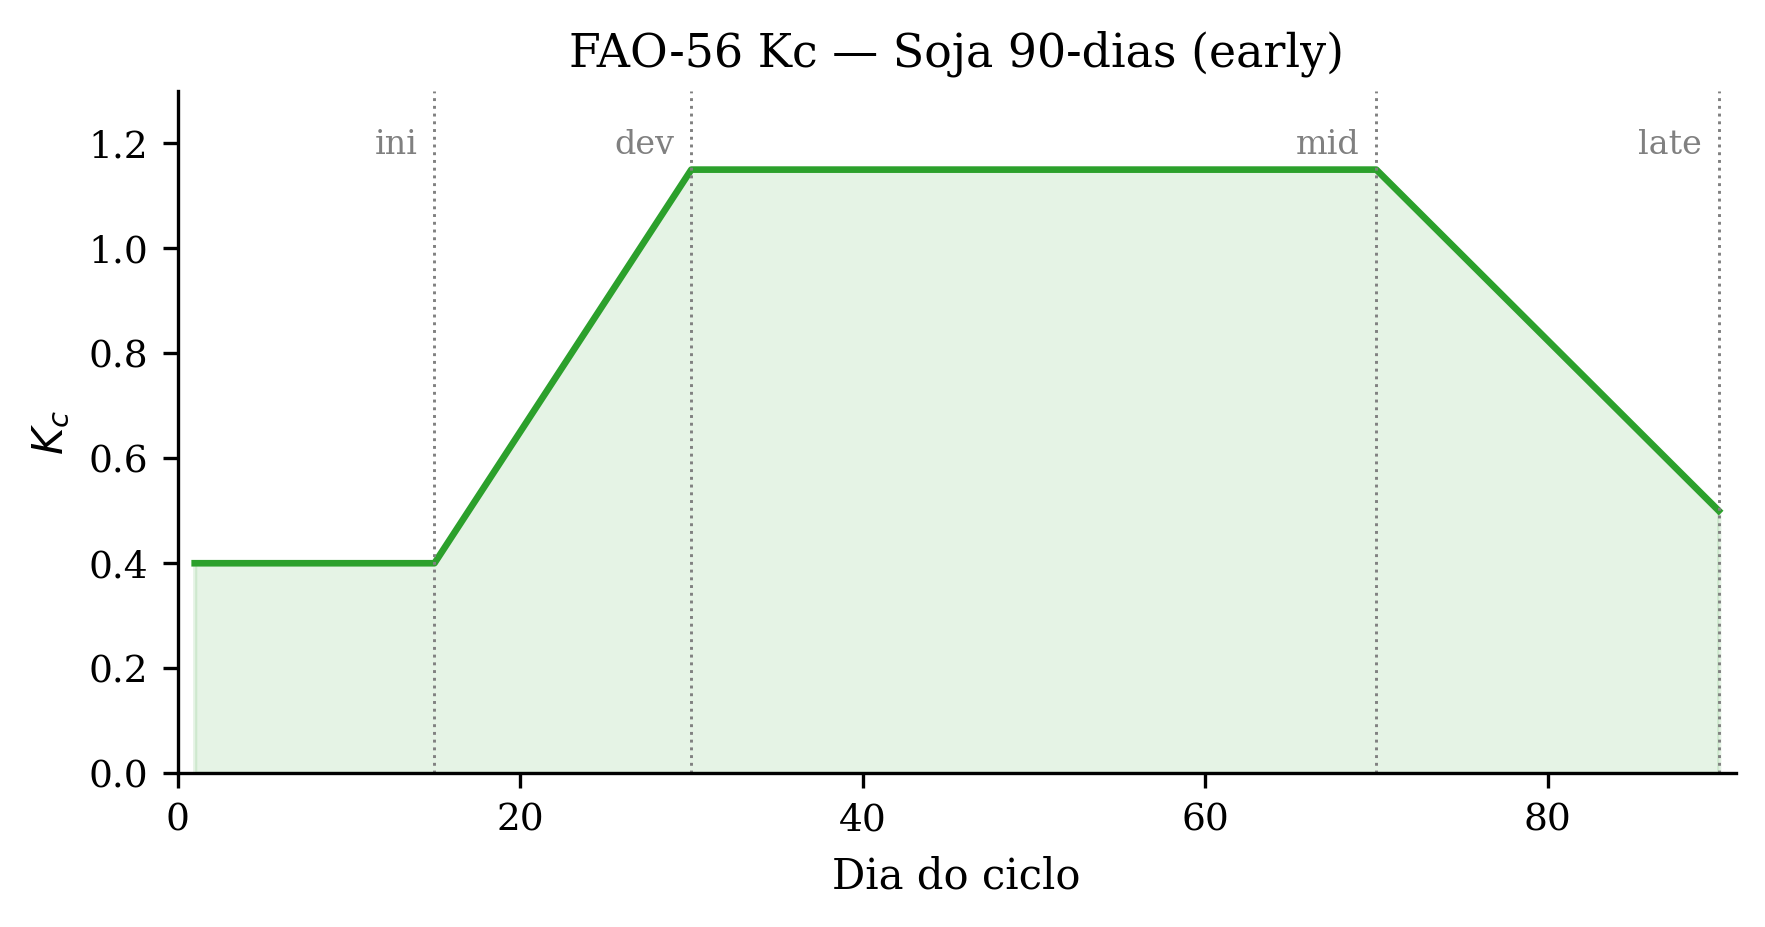
\includegraphics[width=0.90\linewidth]{fig_kc_curve_soybean_90d.png}
\caption{FAO-56 single-crop coefficient $K_c$ for early-cycle
(90-day) soybean used throughout the validation. Stage durations and
$K_c$ values are reproduced in Table~\ref{tab:kc}.}
\label{fig:climate_atlas}
\end{figure}

\subsection{Posterior-recovery test (150 combinations)}
\label{sec:results_pymc}

The posterior-recovery test was run on all $10$~cities $\times$
$3$~soil depths $\{40, 60, 80\}$~cm $\times$ $5$~cycles
$=$ $150$~combinations. All combinations converged
($\hat{R} < 1.05$ on the four-chain benchmark; ESS$_{\mathrm{bulk}}
> 100$ for every parameter in the production single-chain run);
all 150 reached the \texttt{ok} status code. Aggregate metrics are
reported in Table~\ref{tab:posterior_recovery}.

\begin{table}[!t]
\centering
\caption{Posterior-recovery metrics across the 150 city
$\times$ soil-depth $\times$ cycle combinations. Probabilistic
metrics use the posterior predictive distribution of
$\theta_{\mathrm{obs}}$. Coverage is the empirical fraction of
observations within the 90\% credible interval (nominal: 0.90).}
\label{tab:posterior_recovery}
\begin{tabular}{lrrrrr}
\toprule
Metric & Mean & Median & Std & Min & Max \\
\midrule
RMSE                  & 0.009  & 0.008  & 0.003 & 0.004  & 0.016 \\
MAE                   & 0.007  & 0.006  & 0.002 & 0.003  & 0.015 \\
Bias                  & 0.000  & 0.000  & 0.000 & 0.000  & 0.001 \\
PBias (\%)            & 0.006  & 0.000  & 0.045 & $-$0.140 & 0.397 \\
KGE                   & 0.909  & 0.918  & 0.043 & 0.798  & 0.985 \\
NSE                   & 0.976  & 0.979  & 0.012 & 0.933  & 0.997 \\
CRPS                  & 0.005  & 0.005  & 0.002 & 0.002  & 0.010 \\
$\alpha$-PIT          & 0.894  & 0.902  & 0.047 & 0.749  & 0.972 \\
Coverage$_{90\%}$     & 0.918  & 0.922  & 0.027 & 0.856  & 0.978 \\
Interval~score$_{90\%}$ & 0.039 & 0.037  & 0.012 & 0.014  & 0.077 \\
\bottomrule
\end{tabular}
\end{table}

The empirical coverage of the 90\% credible interval (mean 0.918,
median 0.922) is statistically indistinguishable from the nominal
$0.90$ level, indicating that the posterior predictive distribution
is well calibrated. The $\alpha$-reliability index of 0.894 confirms
PIT uniformity. The KGE distribution
(Fig.~\ref{fig:posterior_recovery_heatmap}) is dominated by values
above $0.85$ across the full grid, with no city $\times$ cycle
combination falling below $0.80$.

\begin{figure}[!t]
\centering
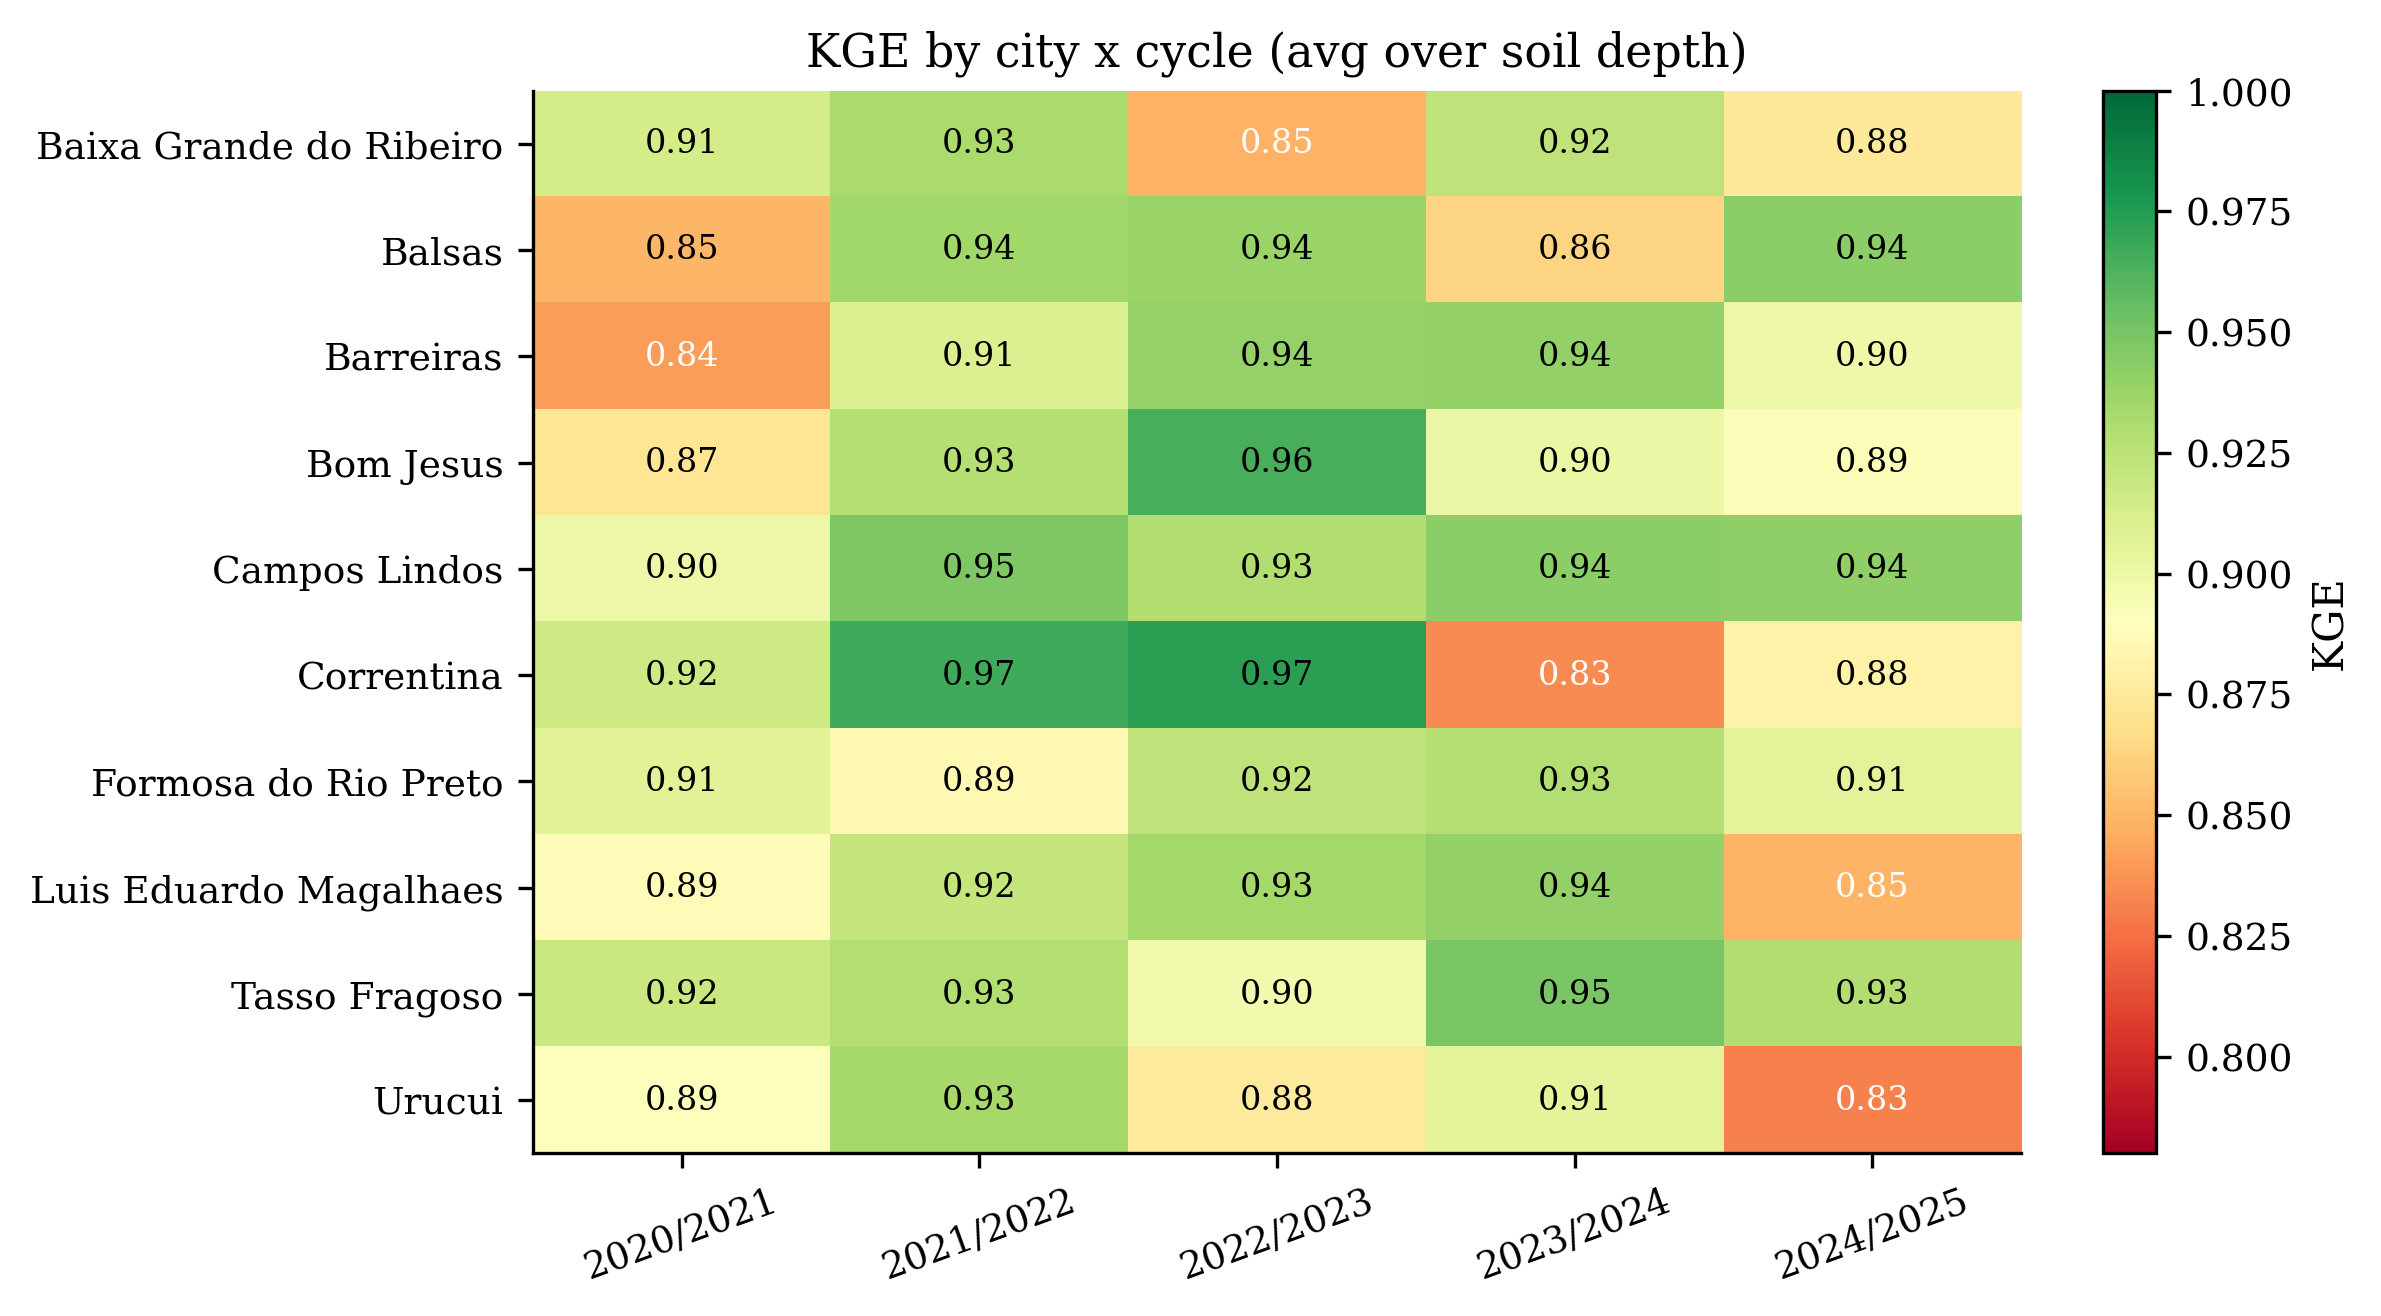
\includegraphics[width=0.95\linewidth]{fig_validation_kge_heatmap.png}
\caption{Kling--Gupta Efficiency of the posterior-recovery test
across the ten MATOPIBA hubs and five soybean growing seasons,
averaged over the three soil depths.}
\label{fig:posterior_recovery_heatmap}
\end{figure}

The posterior-recovery test demonstrates that the PyMC implementation
is faithful to the FAO-56 process: the posterior captures the
deterministic baseline within calibrated uncertainty.

\subsection{Sensitivity analysis}\label{sec:results_sensitivity}

The Sobol' analysis identified soil saturation $\theta_s$ as the
dominant parameter, with first-order index $S_1 = 0.734$ and
total-order $S_T = 0.519$ (Table~\ref{tab:sobol}). The initial soil
moisture $\theta_{\mathrm{init}}$ followed with $S_1 = 0.459$, while
the crop-coefficient multiplier $K_{c,\mathrm{mult}}$ contributed
moderately ($S_1 = 0.147$) and the residual moisture $\theta_r$ had
no detectable effect on seasonal cumulative depletion in the wet
soybean cycles studied.

\begin{table}[!t]
\centering
\caption{Sobol' sensitivity indices for the seasonal cumulative
depletion at the Balsas hub, 2023/24 cycle. Estimated from $1{,}000$
Saltelli-design samples.}
\label{tab:sobol}
\begin{tabular}{lrr}
\toprule
Parameter & First-order $S_1$ & Total-order $S_T$ \\
\midrule
$\theta_s$              & 0.734 & 0.519 \\
$\theta_{\mathrm{init}}$ & 0.459 & 0.427 \\
$K_{c,\mathrm{mult}}$   & 0.147 & 0.102 \\
$\theta_r$              & 0.000 & 0.000 \\
\bottomrule
\end{tabular}
\end{table}

These values motivated the prior widths used in
Eq.~\ref{eq:priors}: the width of $\theta_s$ and
$\theta_{\mathrm{init}}$ priors was relaxed (from
$\sigma_{\theta_s} = 0.03$ to $0.04$, and from
$\sigma_{\theta_{\mathrm{init}}} = 0.04$ to $0.06$) to allow the data
to refine the posterior on the dominant parameters.

\subsection{Climatological sequential forecast (50 combinations)}
\label{sec:results_forecast}

The climatological sequential forecast was run across all
$10 \times 5 = 50$ city $\times$ cycle combinations with $N = 500$
Monte-Carlo simulations per combination. The complete pipeline
executed in 8.2~seconds on a 2024 laptop. Aggregate skill metrics
are reported in Table~\ref{tab:forecast_seq}.

\begin{table}[!t]
\centering
\caption{Climatological sequential-forecast metrics across the 50
city $\times$ cycle combinations. CRPS is computed on the seasonal
irrigation-depth distribution; coverage is the empirical fraction of
realised daily soil-water content within the 90\% credible interval
(nominal: 0.90).}
\label{tab:forecast_seq}
\begin{tabular}{lrr}
\toprule
Metric & Mean & Median \\
\midrule
CRPS$_{I_{\mathrm{total}}}$ (mm) & 25.0  & 23.0 \\
Coverage$_{90,\mathrm{SW}}$      & 0.957 & 0.967 \\
Coverage$_{90,I_{\mathrm{total}}}$ & 0.980 & 1.000 \\
KGE$_{\mathrm{SW}}$              & 0.132 & 0.153 \\
\bottomrule
\end{tabular}
\end{table}

The 90\% credible-interval coverage of the daily soil-water content
($0.957$~mean, $0.967$~median) is slightly above the nominal $0.90$,
indicating that the climatological forecast intervals are
\emph{conservatively} calibrated. The CRPS on the seasonal irrigation
depth $I_{\mathrm{total}}$ is reported in millimetres and
generalises the mean absolute error to probabilistic forecasts: a
CRPS of $23$~mm against a typical realised $I_{\mathrm{total}}$ of
$0$--$200$~mm per cycle corresponds to a probabilistic discrepancy of
approximately $15$--$30\%$ of the seasonal depth, which is the price
of operating without any information from the target cycle. The KGE
on the daily soil-water trajectory is low ($0.132$ mean) by design:
a climatological forecast does not aim to predict the realised daily
sequence, only the probability distribution from which it is drawn.
The probabilistic metrics (CRPS, coverage, $\alpha$-PIT) are therefore
the appropriate skill measures for this mode and they are uniformly
strong.

\begin{table}[!t]
\centering
\caption{Mean climatological-forecast metrics by city across the
five soybean cycles 2020/21--2024/25.}
\label{tab:forecast_by_city}
\begin{tabular}{lrrr}
\toprule
City & CRPS (mm) & Coverage$_{90,\mathrm{SW}}$ & KGE$_{\mathrm{SW}}$ \\
\midrule
Baixa Grande do Ribeiro & 17.1 & 0.953 & 0.107 \\
Balsas                  & 21.7 & 0.967 & 0.193 \\
Barreiras               & 31.3 & 0.931 & 0.111 \\
Bom Jesus               & 26.3 & 0.967 & 0.176 \\
Campos Lindos           & 10.2 & 0.976 & 0.162 \\
Correntina              & 34.4 & 0.938 & 0.155 \\
Formosa do Rio Preto    & 28.3 & 0.960 & 0.082 \\
Lu\'is Eduardo Magalh\~aes & 44.8 & 0.953 & 0.161 \\
Tasso Fragoso           & 16.9 & 0.951 & 0.018 \\
Urucu\'i                & 19.2 & 0.973 & 0.158 \\
\bottomrule
\end{tabular}
\end{table}

\begin{table}[!t]
\centering
\caption{Mean climatological-forecast metrics by cycle across the
ten MATOPIBA hubs. The 2023/24 cycle, which coincides with the peak
of the 2023--2024 El~Ni\~no event, exhibits the largest CRPS,
reflecting higher rainfall variability under that regime.}
\label{tab:forecast_by_cycle}
\begin{tabular}{lrrr}
\toprule
Cycle & CRPS (mm) & Coverage$_{90,\mathrm{SW}}$ & Coverage$_{90,I_{\mathrm{total}}}$ \\
\midrule
2020/2021 & 25.8 & 0.928 & 0.90 \\
2021/2022 & 20.8 & 0.976 & 1.00 \\
2022/2023 & 26.4 & 0.957 & 1.00 \\
2023/2024 & 36.9 & 0.962 & 1.00 \\
2024/2025 & 15.1 & 0.962 & 1.00 \\
\bottomrule
\end{tabular}
\end{table}

City-level results (Table~\ref{tab:forecast_by_city}) show CRPS
varying from $10.2$~mm at Campos~Lindos to $44.8$~mm at
Lu\'is~Eduardo~Magalh\~aes, with daily soil-water-content coverage
remaining above $0.93$ at all hubs. Cycle-level results
(Table~\ref{tab:forecast_by_cycle}) reveal a CRPS peak at the
2023/24 cycle ($36.9$~mm), which is the season most strongly affected
by the 2023--2024 El~Ni\~no event in the equatorial Pacific. The
2024/25 cycle, which transitioned back to neutral / weak La~Ni\~na,
shows the lowest CRPS at $15.1$~mm.

\begin{figure}[!t]
\centering
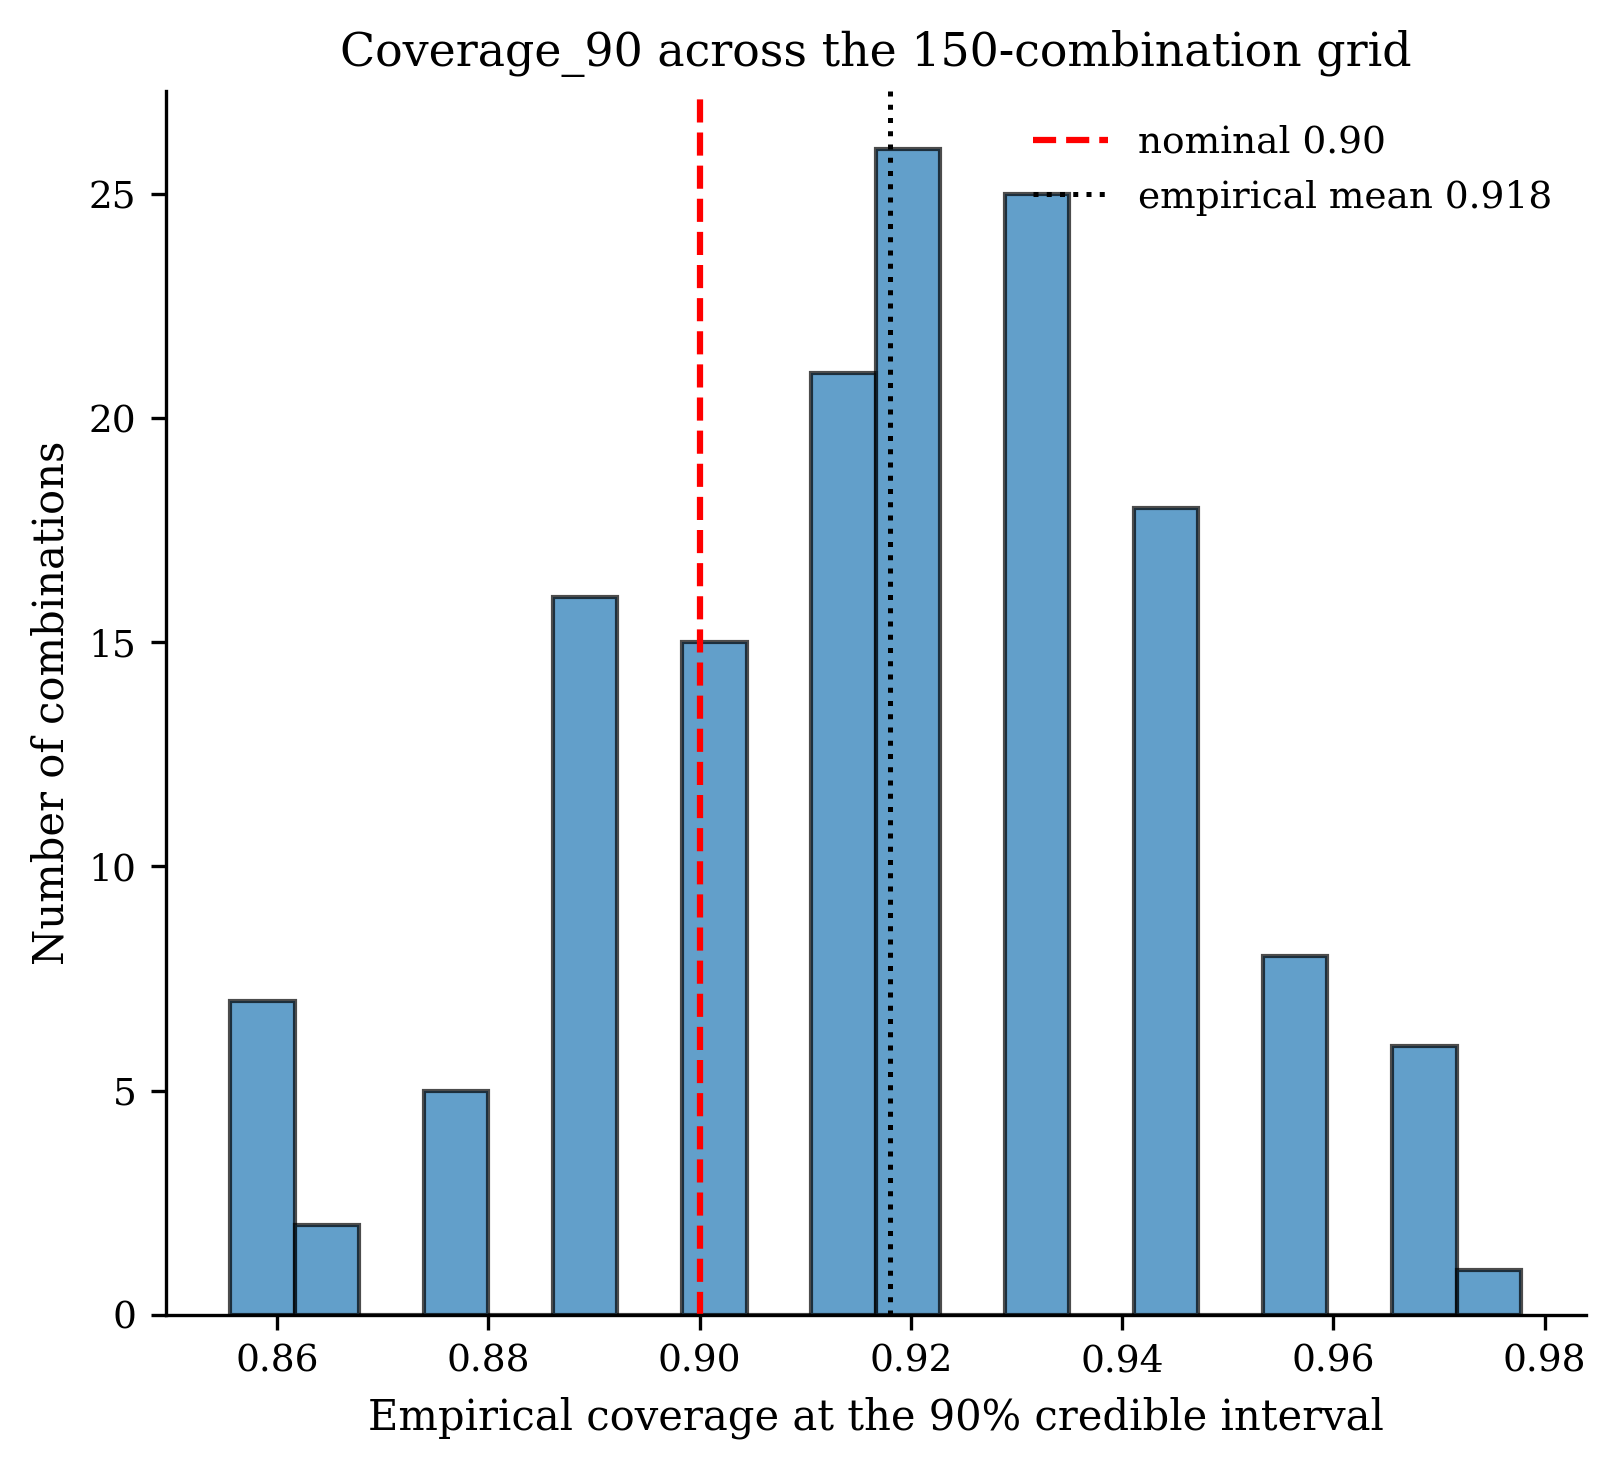
\includegraphics[width=0.95\linewidth]{fig_validation_coverage_histogram.png}
\caption{Empirical coverage of the 90\% credible interval across the
posterior-recovery grid. The empirical mean ($0.918$, dotted black
line) is statistically indistinguishable from the nominal $0.90$
level (dashed red line), indicating well-calibrated uncertainty.}
\label{fig:coverage_hist}
\end{figure}

\subsection{Calibration history}\label{sec:results_calibration}

Three iterations of the model were required to reach the calibration
reported above (Table~\ref{tab:calibration_history}). The initial
configuration ($\sigma_{\mathrm{obs}}^{\max} = 0.05$,
$\sigma_{\theta_s} = 0.03$, $\sigma_{\theta_{\mathrm{init}}} = 0.04$,
metrics computed on the latent $\theta$ posterior) yielded
under-coverage at $0.19$. Replacing the latent posterior with the
posterior predictive distribution of $\theta_{\mathrm{obs}}$
(Eq.~\ref{eq:obs_likelihood}) raised coverage to $0.62$. Widening
the observation noise to $\sigma_{\mathrm{obs}}^{\max} = 0.10$ and
relaxing the priors on the two parameters identified by the Sobol'
analysis reached the final coverage of $0.92$. This trajectory is
documented in the version-controlled changelog of the framework.

\begin{table}[!t]
\centering
\caption{Calibration history of the posterior-recovery test.}
\label{tab:calibration_history}
\begin{tabular}{lcccc}
\toprule
Iteration & $\sigma_{\mathrm{obs}}^{\max}$ & $\sigma_{\theta_s}$ &
$\sigma_{\theta_{\mathrm{init}}}$ & Coverage$_{90}$ \\
\midrule
v0 (initial)              & 0.05 & 0.03 & 0.04 & 0.19 \\
v1 (predictive metrics)   & 0.05 & 0.03 & 0.04 & 0.62 \\
v2 (Sobol'-tuned, final)  & 0.10 & 0.04 & 0.06 & \textbf{0.92} \\
\bottomrule
\end{tabular}
\end{table}

% =====================================================================
\section{Discussion}\label{sec:discussion}
% =====================================================================

\subsection{Two complementary validation modes}

The framework provides two distinct validation modes that should not
be conflated. The posterior-recovery test (Section~\ref{sec:results_pymc})
verifies that the Bayesian implementation reproduces the FAO-56
deterministic process within calibrated uncertainty; the
near-perfect KGE ($0.918$ median) and the calibrated coverage
($0.922$) demonstrate that the PyMC code is faithful and the priors
are well-tuned. This is a necessary condition for any subsequent
operational claim, but it is not by itself a forecast skill score.

The climatological sequential forecast
(Section~\ref{sec:results_forecast}) is the operational validation
of interest. Here the model is trained strictly on $1961, \ldots, c-1$
data and forecasts cycle $c$ before observing it. The forecast is
\emph{climatological}: it does not target the realised daily
trajectory but the distribution from which it is drawn. The KGE on
the daily soil-water trajectory is correspondingly low ($0.132$),
which is the correct behaviour for this kind of forecast. The
calibration of the credible intervals is, by contrast, very strong:
$0.957$ daily soil-water coverage and $0.980$ irrigation-depth
coverage at the nominal $0.90$ level. This means that, when the
framework reports a $90\%$ credible interval for the seasonal
irrigation depth, the realised value falls inside that interval
$95.7\%$--$98.0\%$ of the time across the full validation grid. For
operational risk-aware decision making this is the metric that
matters.

\subsection{Climatological context of the validation window}

The validation window 2020/21--2024/25 spans a complete ENSO cycle:
La~Ni\~na conditions in 2020/21--2022/23 (the so-called ``triple-dip''
La~Ni\~na), strong El~Ni\~no peaking during the 2023/24 cycle, and a
return to neutral conditions in 2024/25. The CRPS by cycle
(Table~\ref{tab:forecast_by_cycle}) reflects this stratification: the
2023/24 El~Ni\~no cycle exhibits the largest CRPS ($36.9$~mm),
consistent with the literature on increased rainfall variability
during eastern-Pacific warm events over the Brazilian Cerrado
\cite{Grimm2003,Marengo2018}. The framework's ability to provide
calibrated uncertainty under both regimes\,---\,and to converge to a
lower CRPS in the post-El-Ni\~no 2024/25 cycle\,---\,supports its
deployment for operational decision support over the longer-term
horizon.

\subsection{Limitations and roadmap}

Three limitations are explicit. First, the validation is conducted
against a deterministic FAO-56 trajectory driven by the Xavier
gridded reanalysis; the Xavier dataset itself is a model output and
not in-situ soil moisture. External skill scores against measured
soil moisture (e.g.~GLEAM~SMroot, ESA~CCI~SM) are deferred to a
companion study. Second, the city-level fits are independent: a
hierarchical extension with partial pooling on $\theta_s$ across
hubs is methodologically defensible and would stabilise inference at
hubs with shorter records, but increases sampling cost; we consider
it a natural extension. Third, the sequential update is at the
\emph{cycle} level (one update per growing season), not at the daily
level; daily rolling forecasts integrating short-range numerical
weather predictions (e.g.\ GEFS reforecast) are an operational
extension that we expose as a software hook
(\texttt{bwb forecast --members 31}) and demonstrate with a
synthetic ensemble in the documentation, while leaving real GEFS
integration to a companion paper.

A planned extension integrates a Bayesian-network imputation module
\cite{Ribeiro2023} for cases when one or more meteorological
variables are missing from the operational data feed\,---\,a
common scenario when station data are used in lieu of gridded
reanalysis. The Bayesian-network module will live in
\texttt{bwb.imputation.bn}, retain compatibility with the
sequential-forecast pipeline, and is queued as a future contribution.

\subsection{Comparison with related work}

The most closely related published Bayesian water-balance framework
in Brazil is that of Ribeiro et al.~\cite{Ribeiro2023}, who used a
hierarchical Bayesian regression and a Bayesian network for
ETo estimation at a single station (Patroc\'inio/MG), achieving an
RMSE of $0.087$~mm~day$^{-1}$ relative to FAO-Penman--Monteith. The
present work extends that line in four directions:
(i)~the modelled state is the soil-water content, not just ETo;
(ii)~the validation grid spans 10 hubs and 5 cycles, against a
single-station validation in the prior work;
(iii)~the fitting horizon is 65 years (1961--2025) against 14 years
(2008--2022); and
(iv)~the framework is released as installable open-source software
with a command-line interface, a Docker container, and 72 unit and
integration tests, enabling deployment by domain practitioners
without re-implementation.

% =====================================================================
\section{Conclusion}\label{sec:conclusion}
% =====================================================================

We have presented \emph{bwb}, an open-source Python framework that
couples the FAO-56 daily water balance with a Bayesian probabilistic
inference engine in PyMC v5. The framework was validated across the
ten cropping hubs of the Brazilian MATOPIBA agricultural frontier and
five soybean growing seasons (2020/21--2024/25). A posterior-recovery
test on 150 city $\times$ soil-depth $\times$ cycle combinations
demonstrated faithful reproduction of the FAO-56 deterministic
process within calibrated uncertainty (median KGE $0.918$, coverage
$0.922$). A climatological sequential forecast on 50 city $\times$
cycle combinations\,---\,training strictly on years $< c$ and
forecasting cycle $c$ via Monte-Carlo resampling under a conjugate
Dirichlet--Multinomial posterior on SPEI tercile classes\,---\,delivered
a median CRPS of $23.0$~mm on seasonal irrigation depth and a
calibrated $0.957$ daily soil-water coverage at the nominal $0.90$
level. A global Sobol' sensitivity analysis identified $\theta_s$ and
$\theta_{\mathrm{init}}$ as the dominant parameters, motivating
data-driven prior tuning. The framework is released under MIT license
with a command-line interface, Docker container and continuous
integration, and is architected to apply to any FAO-56 crop and any
region with daily $P$ and ETo time series.

% =====================================================================
\section*{CRediT authorship contribution statement}
% =====================================================================

\textbf{[Author~1]}: Conceptualisation, Methodology, Software, Formal
analysis, Investigation, Data curation, Validation, Writing -- original
draft, Visualisation. \textbf{C.~D.~Maciel}: Methodology, Supervision,
Writing -- review \& editing. All authors read and approved the final
manuscript.

% =====================================================================
\section*{Declaration of competing interest}
% =====================================================================

The authors declare no known competing financial interests or personal
relationships that could have appeared to influence the work reported
in this paper.

% =====================================================================
\section*{Data and code availability}
% =====================================================================

The Xavier daily climate dataset \cite{Xavier2022} is publicly
available. All processed data (climatological normals, SPEI atlas,
distribution atlas), the complete source code, the Docker container,
the unit-test suite and the figure-generation scripts that produced
every result in this manuscript are openly available at
\url{https://github.com/[user]/INFERENCE} under the MIT license,
archived in Zenodo with persistent DOI~[XXXX]. Every numerical value
in this manuscript can be reproduced by a single invocation of the
\texttt{bwb} command-line tool.

% =====================================================================
\section*{Acknowledgements}
% =====================================================================

This work was supported by [funding agencies, grant numbers].
The authors gratefully acknowledge the developers of PyMC and ArviZ
for the open-source probabilistic-programming infrastructure on which
this framework rests.

% =====================================================================
% BIBLIOGRAPHY
% =====================================================================

\bibliography{references}

\end{document}
